% V2 submission — ARR/ACL anonymous review format.
% Built from v2_quality/paper/manuscript.md (same scientific content).
% Sources: immutable F1/F2 CSV/JSON + frozen V1 locked study. No content
% from paper/phase21_tables.md (known numerical errors).

\documentclass[11pt]{article}
\usepackage[review]{acl}
\usepackage{times}
\usepackage{graphicx}
\usepackage{booktabs}
\usepackage{latexsym}
\usepackage{multirow}
\usepackage{array}
\usepackage{amsmath}
\usepackage{xurl}

\title{When Does Task-Conditioned Cognitive Configuration Search\\
Generalize? A Controlled Audit of LLM Agent Scaffolds with Fair\\
Baselines, Token Costs, and a Cross-Benchmark Test}

\author{Anonymous ARR submission}
\date{}

\begin{document}
\maketitle

\begin{abstract}
LLM agents are usually deployed with a fixed, hand-designed cognitive
configuration: a reasoning strategy, an episodic memory/exemplar policy,
and a context budget chosen once and reused across tasks. We ask a narrower
and more auditable question than ``can we evolve better agents'': do
task-conditioned choices of these configuration components materially
change accuracy and inference cost above a frozen backbone, and does
automatic search over them find configurations whose advantage survives
fair baselines and unseen data? We study this with a three-tier audit of
QA-style single-agent scaffolds over frozen Qwen2.5 backbones, keeping
every tier's evidence status explicit. \textbf{Tier 1} (previously locked,
descriptive): on an untouched GSM8K holdout, a search-selected
chain-of-thought (CoT) configuration outperformed four fixed baselines that
all used direct answering, by +29.0 percentage points at 1.5B and +16.7
points at 7B---an architecture-matters result that confounds search with
the CoT-vs-direct gap and cannot be attributed to search alone.
\textbf{Tier 2} (fair-baseline dev audit): against CoT-matched presets on
the reused GSM8K dev slice, the search-selected configuration shows no
statistically detectable accuracy advantage over the strongest preset
(60.0\% vs 59.0\%, $+1.0$pp, $p{=}1.0$); its +10-point edge over a
no-memory CoT control is exploratory ($p{=}0.087$). \textbf{Tier 3}
(pre-locked cross-benchmark confirmation): on 300 locked SVAMP test items
never used for search or tuning, the search-selected configuration scores
70.33\%, with no statistically detectable accuracy difference from either
the strong CoT preset
(71.67\%; primary contrast $-1.33$pp, 95\% CI $[-6.00, +3.33]$, exact
McNemar $p{=}0.67$) and the no-memory control (70.33\%; $0.00$pp,
$p{=}1.0$)---and the dev-side memory benefit does not replicate. Cost
analysis is equally blunt: the no-memory control matches the searched
configuration's observed accuracy with 1.75$\times$ fewer total tokens.
Equal-budget evolutionary search also does not beat random search in our
compact audited space, and a correctly implemented trainable Mamba-2
substrate is not selected as beneficial. Our contribution is not a new
optimizer but a falsifiable audit protocol---fair CoT-matched baselines,
item-level paired statistics, total-token cost accounting, and a pre-locked
cross-benchmark confirmation---together with its two-sided findings.
\end{abstract}

\section{Introduction}

Assembling an LLM agent involves choices that are usually made by hand and
then frozen: whether to reason directly or step by step, whether to carry
an episodic memory of exemplars and in what form, and how much of the
context budget to spend on them. A growing line of work automates these
choices---searching agent programs, modular designs, or multi-agent
topologies---and typically reports that the searched artifact beats the
manual one on the benchmark used for searching. What is audited far less
often is whether such advantages survive two elementary controls: (i)
baselines matched on the \emph{components} the search actually varies, and
(ii) evaluation on data the search never touched.

This paper reports such an audit for task-conditioned \emph{cognitive
configuration search}: per-task selection of a reasoning strategy, an
episodic memory/exemplar policy, and a context allocation policy above a
frozen backbone. Our setting is deliberately modest---QA-style single-agent
scaffolds, not interactive tool-using or multi-agent systems, and not
neural architecture search over backbone weights---because the audit
questions are already sharp there, and because leakage-safe paired
evaluation is feasible at that scale.

We organize the evidence into three tiers with explicitly different
epistemic status. \textbf{Tier 1} is a previously locked holdout study
(frozen before this paper): its headline---a searched configuration beating
the strongest fixed baseline by +29.0 percentage points at 1.5B and +16.7
at 7B on GSM8K holdout---is real but descriptive, because all four fixed
baselines used direct answering while the searched configuration used CoT.
\textbf{Tier 2} repairs baseline fairness: CoT-matched presets compared
against the search-selected configuration on the same dev slices the search
used (exploratory by construction). \textbf{Tier 3} is a pre-locked
confirmation: three configurations frozen before any inference, evaluated
once on the 300-item original SVAMP test split, a public benchmark never
used for search, calibration, or tuning.

The findings are two-sided. Configuration choices matter: reasoning
strategy alone swings GSM8K dev accuracy from 11\% (direct) to 50--60\%
(CoT), and CoT variants span ${\sim}8.3\times$ in prompt tokens with
observed accuracies of 49--60\%. But the search-selected configuration shows no detectable
advantage over a strong hand-picked CoT preset on either the dev slice or
the locked SVAMP test; its dev-side +10-point benefit over a no-memory
control does not replicate cross-benchmark ($0.00$pp, $p{=}1.0$); the
cheapest control matches its observed SVAMP accuracy with 1.75$\times$
fewer total tokens; and, in the compact space where we enumerated the full
landscape, equal-budget evolutionary search does not outperform random
search. We report all of this---including the negative results---as the
contribution: a protocol that makes configuration-search claims
falsifiable, and a precise map of which claims survived it.

\section{Related Work}

\paragraph{Automated agent design.} ADAS~\citep{hu2024adas} searches over
agent programs expressed in code; AgentSquare~\citep{shang2025agentsquare}
searches a modular design space of planning, reasoning, tool-use, and
memory modules; MaAS~\citep{zhang2025maas} performs query-dependent
multi-agent architecture search through an agentic supernet and explicitly
prices inference resources. These systems optimize performance (MaAS also
cost) on the search distribution. We differ in target and emphasis: our
search target is the internal cognitive configuration of a single
frozen-backbone agent, and our main object of study is the gap between
search-side selection and held-out, fair-baseline, cross-benchmark
evidence---including where the search procedure itself fails to beat random
search. Evo-Memory~\citep{wei2025evomemory} and related work study
continually evolving agent memory during deployment; here memory is not
evolved online---the memory policy is one component of a task-conditioned
configuration searched against a fixed, calibration-only experience bank.
DSPy~\citep{khattab2023dspy} compiles declarative LLM programs into
optimizable pipelines; EvoPrompt~\citep{guo2024evoprompt} evolves prompt
text. We treat reasoning strategy as one gene jointly audited with memory
and context policy.

\paragraph{Scaffolds and prompting.} ReAct~\citep{yao2023react},
Reflexion~\citep{shinn2023reflexion}, and chain-of-thought
prompting~\citep{wei2022cot} are hand-designed cognitive configurations in
our terms; verification and planning variants appear as reasoning genes.
Retrieval-augmented generation~\citep{lewis2020rag} grounds LLMs in
external evidence; our memory policies manage a leakage-safe,
calibration-only exemplar bank, and we quantify when such memory helps,
hurts, or is neutral.

\paragraph{Search methodology.} Our evolutionary loop follows regularized
evolution~\citep{real2019ameoba} and NSGA-II-style non-dominated sorting
with crowding distance~\citep{deb2002nsga2}; Bayesian optimization is the
standard sample-efficiency reference~\citep{snoek2012bayesopt};
AlphaEvolve~\citep{alphaevolve2025} shares the evolutionary loop but
evolves programs. Unlike NAS over backbone weights, our search operates
above a frozen LLM, and we enumerate the compact space exhaustively so
evolutionary search can be audited against equal-budget random search on a
known landscape. Mamba~\citep{gu2023mamba} and
Mamba-2~\citep{dao2024mamba2} provide the selective state-space models
behind our trainable memory substrate, which is implemented and searchable
but---as we report---not selected as beneficial.

\paragraph{Evaluation.} We use GSM8K~\citep{cobbe2021gsm8k},
SVAMP~\citep{patel2021svamp}, PubMedQA~\citep{jin2019pubmedqa}, and
QASPER~\citep{dasigi2021qasper} in its LongBench form~\citep{bai2023longbench}
with frozen Qwen2.5-Instruct backbones~\citep{yang2024qwen25}. We claim no
priority over any of the above; the contribution is the audit protocol and
its two-sided findings.

\section{Setting and Audit Design}

\paragraph{Cognitive configuration space.} A configuration is a structured
genome over three gene families: (i) \emph{memory policy}---none / recency
/ retrieval (term-frequency cosine or hashed bag-of-words cosine over a
calibration-only exemplar bank) / a trainable Mamba-2 substrate / hybrid,
with recall width and exemplar-count sub-genes; (ii) \emph{reasoning
strategy}---direct, chain-of-thought (with depth), verify, planner; (iii)
\emph{context policy}---full, truncated, or answer-only exemplar verbosity
with word budgets. Normalization removes semantically inactive sub-genes
before hashing so duplicate phenotypes are never double-counted. A compact
audit layer (memory $\times$ reasoning $\times$ context $=$ 48
configurations) is fully enumerated per benchmark as a ground-truth
landscape.

\paragraph{Three evidence tiers.}
\textbf{Tier 1---locked descriptive holdout (frozen).} Pre-specified,
commit-locked holdout evaluation of task-selected configurations vs four
fixed baselines (all direct-answering) on GSM8K/PubMedQA/QASPER, plus the
exhaustive-landscape search-efficiency audit; locked before this paper and
reported with confounds made explicit.
\textbf{Tier 2---fair-baseline dev audit.} Six predefined baselines (four
CoT-matched and two Direct controls) matched to the search-selected
configuration's reasoning strategy, plus the search-selected REF itself,
run on the same dev slices the search used (GSM8K test$[0{:}100]$, QASPER items$[0{:}50]$) and
a pre-chosen 7B shortlist; exploratory, with provenance gaps (\S\ref{sec:tier2}).
\textbf{Tier 3---pre-locked cross-benchmark confirmation.} Three
configurations (search-selected REF, strongest CoT preset B2, no-memory CoT
control B1) frozen with all 300 SVAMP test IDs, file hashes, model
revision, and analysis plan \emph{before any inference}; evaluated exactly
once; primary and secondary contrasts fixed in advance. Independent of the
project's selection history, but a public benchmark (pretraining
contamination cannot be ruled out) and not same-distribution with GSM8K.

\paragraph{Statistics.} All key comparisons are paired at the item level
with paired bootstrap 95\% CIs (10{,}000 resamples, fixed seed). For binary
outcomes (GSM8K, SVAMP, PubMedQA), significance uses two-sided exact
McNemar tests; for continuous QASPER item-level F1, a two-sided exact
paired sign test over non-tied differences. Absence of significance is not
treated as equivalence.

\paragraph{Scope.} These are QA-style single-agent cognitive scaffolds
above a frozen LLM. We do not evaluate interactive tool-using, multi-agent,
embodied, or long-horizon environment agents, and our conclusions do not
directly extend to them.

\section{Tier 1 --- Locked Descriptive Holdout: Architecture Matters, Search Credit Unclear}
\label{sec:tier1}

The frozen pre-study (pre-specified, commit-locked before holdout
inference) task-searched configurations on dev slices and evaluated once on
untouched holdouts (GSM8K test$[100{:}1319]$; PubMedQA 400 items; QASPER
100 items; Qwen2.5-1.5B/7B).

\paragraph{Headline, with its confound.} On GSM8K holdout the
search-selected configuration (recency memory, CoT depth 3, full context)
reaches 0.518 at 1.5B and 0.859 at 7B, beating the strongest fixed baseline
by +29.0 and +16.7 percentage points (McNemar $p{<}0.001$). However, all
four fixed baselines answered \emph{directly}; the searched configuration
used CoT. The gap is therefore best read as ``cognitive architecture
choices matter materially,'' not as isolated evidence for search or for
memory: Tier 2 shows CoT-matched presets close most of it.

\paragraph{Search-side selection.} Task-conditioned preferences were stable
and interpretable: GSM8K consistently favored CoT-style reasoning across
seeds (3/3, depth 2--3) with the lightweight memory choice varying among
none/recency/retrieval; PubMedQA converged bit-identically to no-memory
direct answering; QASPER shifted the optimum toward retrieval memory with
many exemplars---a pre-specified prediction that was confirmed. But
dev-selected task-specific configurations did not universally generalize:
on PubMedQA and QASPER holdout they were beaten by the GSM8K-selected
configuration.

\paragraph{Search-efficiency audit (negative).} On the fully enumerated
compact landscape (48 configurations), online evolutionary search does not
beat equal-budget uniform random search at any budget $\{12, 24, 36, 48\}$
on any benchmark (20 seeds; differences below 0.01 in AUC and hypervolume).
We make no optimizer-superiority claim.

\paragraph{Substrate audit (negative).} A real, trainable Mamba-2 memory
substrate participates in the search but is not selected as beneficial.
Controlled same-genome ablations found memory effects to be task- and
scale-dependent (neutral at 1.5B on GSM8K, +12.6pp at 7B; +18.0pp at 1.5B
on PubMedQA; +1.5pp on QASPER); memory causality is claimed only where the
comparison is controlled.

\paragraph{Extraction caveat.} A QASPER configuration that works at 1.5B
shows near-zero extracted-answer F1 at 7B; a frozen diagnostic reveals
perfect marker compliance with the answer placed before the marker---a
backbone--prompt--extraction interaction with a substantial extraction
component. It is not evidence of a pure capability collapse, and the
diagnostic does not establish that underlying answer quality is unaffected.

\section{Tier 2 --- Fair CoT-Matched Baselines on Reused Dev (Exploratory)}
\label{sec:tier2}

Tier 1's fairness gap motivated baselines matched on the searched
configuration's actual components. We evaluated six predefined baselines
(four CoT-matched: B1--B4; two Direct controls: B0/B5) plus the
search-selected REF on GSM8K dev ($n{=}100$) and QASPER dev ($n{=}50$) at
1.5B, with a pre-chosen 7B shortlist (0.16 GPU-hours total;
Table~\ref{tab:f1}).

\begin{table}[t]
\centering\small
\begin{tabular}{@{}lccc@{}}
\toprule
Config & Memory / reasoning & Acc (\%) & Prompt tok \\
\midrule
B0 & none / direct & 11.0 & 6{,}791 \\
B5 & recency$\times$1 / direct & 13.0 & 23{,}091 \\
B1 & none / CoT d3 & 50.0 & 8{,}091 \\
B4 & recency$\times$1, 128w / CoT d3 & 49.0 & 14{,}491 \\
B3 & retrieval tf-cos / CoT d3 & 57.0 & 27{,}683 \\
B2 & recency$\times$3 / CoT d3 & 59.0 & 67{,}391 \\
\textbf{REF} & recency$\times$1 / CoT d3 & \textbf{60.0} & 24{,}391 \\
\bottomrule
\end{tabular}
\caption{GSM8K dev ($n{=}100$, 1.5B), accuracy and prompt-token cost for
the six predefined baselines and the search-selected REF. REF shows no
statistically detectable advantage over the strongest CoT-matched baseline
B2 ($+1.0$pp, exact McNemar $p{=}1.0$); REF$-$B1 $= +10.0$pp (95\% CI
$[0.0, 20.0]$, $p{=}0.087$, exploratory). Direct baselines (B0/B5)
collapse: the Tier-1 headline confounds reasoning strategy with search.}
\label{tab:f1}
\end{table}

\paragraph{GSM8K dev.} Among CoT configurations REF shows no statistically
detectable accuracy difference from B2 or B3 (REF$-$B3 $+3.0$pp,
$p{=}0.63$). The reduced-exemplar-verbosity baseline B4 was lower than REF
on this exploratory dev slice ($+11.0$pp, unadjusted $p{=}0.043$,
secondary); a single contrast on reused dev cannot rank factor importance,
so causal prioritization of context budget over preset choice requires
further controls. The REF$-$B1 gap reflects the memory+exemplar component
under CoT, not search; at 7B (dev, secondary, unadjusted) it is $+10.0$pp
($p{=}0.041$), directionally consistent with Tier-1's scale-dependent
memory ablation but exploratory here.

\paragraph{QASPER dev (exploratory, extraction-sensitive).} REF (0.167) is
slightly \emph{below} B1/B3/B2 (0.184--0.192); paired sign tests are
non-significant. Raw model outputs for these cells were not preserved by
the legacy evaluator---an evidence limitation we carry.

\paragraph{Provenance limitations.} The F1 run manifest covers only the
last four cells (overwrite-on-invocation defect) and records the runner
git SHA as ``unknown'' (VM checkout lacked \texttt{.git}); per-item
prediction files for all 15 cells are committed and were independently
re-scored, but exact runner-source provenance is partially undocumented.
F1 numbers are accepted-with-limitations, not paper-grade confirmation.

\section{Tier 3 --- Pre-Locked SVAMP Confirmation (Single Shot)}
\label{sec:tier3}

\paragraph{Protocol.} Before any inference we committed: all 300 original
SVAMP test IDs in order with file SHA-256s (dataset revision pinned); the
three configurations (REF, B2, B1); the backbone (Qwen2.5-1.5B-Instruct,
exact revision); the Body+Question adapter and numeric scorer (versioned,
unit-tested on synthetic fixtures; Equation/Answer never enter prompts);
the primary contrast (REF vs B2) and secondary (REF vs B1); and the
analysis (paired bootstrap CI + exact McNemar). Memory exemplars came from
the GSM8K \emph{train} calibration bank only; SVAMP train was never read.
Zero normalized exact-match overlap between the 300 locked items and the
full GSM8K corpus was verified pre-inference. A post-hoc read-only forensic
audit re-hashed every committed artifact byte-for-byte (dataset, lock, 900
predictions, paired statistics) and passed, with two honestly annotated
gaps: the run-time loader had checked ordered IDs and count but not full
file bytes (closed post-hoc by the audit), and the on-VM model-revision
observation is not itself a committed artifact.

\begin{table}[t]
\centering\small
\begin{tabular}{@{}lcccc@{}}
\toprule
Config & Acc (\%) & Prompt & Compl. & Total \\
\midrule
REF & 70.33 & 68{,}017 & 50{,}049 & 118{,}066 \\
B2  & \textbf{71.67} & 197{,}017 & 44{,}137 & 241{,}154 \\
B1  & 70.33 & \textbf{19{,}117} & 48{,}264 & \textbf{67{,}381} \\
\bottomrule
\end{tabular}
\caption{Locked SVAMP test ($n{=}300$, 1.5B), single shot. Accuracy in
percent (REF 211/300, B2 215/300, B1 211/300) with prompt, completion, and
total tokens. Primary: REF$-$B2 $= -1.33$pp, 95\% CI $[-6.00, +3.33]$,
exact McNemar $p{=}0.67$. Secondary: REF$-$B1 $= 0.00$pp, CI
$[-5.33, +5.33]$, $p{=}1.0$. B1 matches REF's observed accuracy with
1.75$\times$ fewer total tokens---an observation, not statistically
demonstrated dominance.}
\label{tab:f2}
\end{table}

\paragraph{Results.} One shot, 0 errors, 0.06 GPU-hours
(Table~\ref{tab:f2}, Figure~\ref{fig:scatter}). The search-selected REF
shows \textbf{no detectable advantage} over the strong preset B2; B2 is
nominally $+1.33$pp with 2.04$\times$ REF's total tokens. B1 matches REF's
observed accuracy with 1.75$\times$ fewer total tokens (3.56$\times$ fewer
prompt tokens): in the observed accuracy--token plane REF is dominated by
B1.

\begin{figure*}[t]
\centering
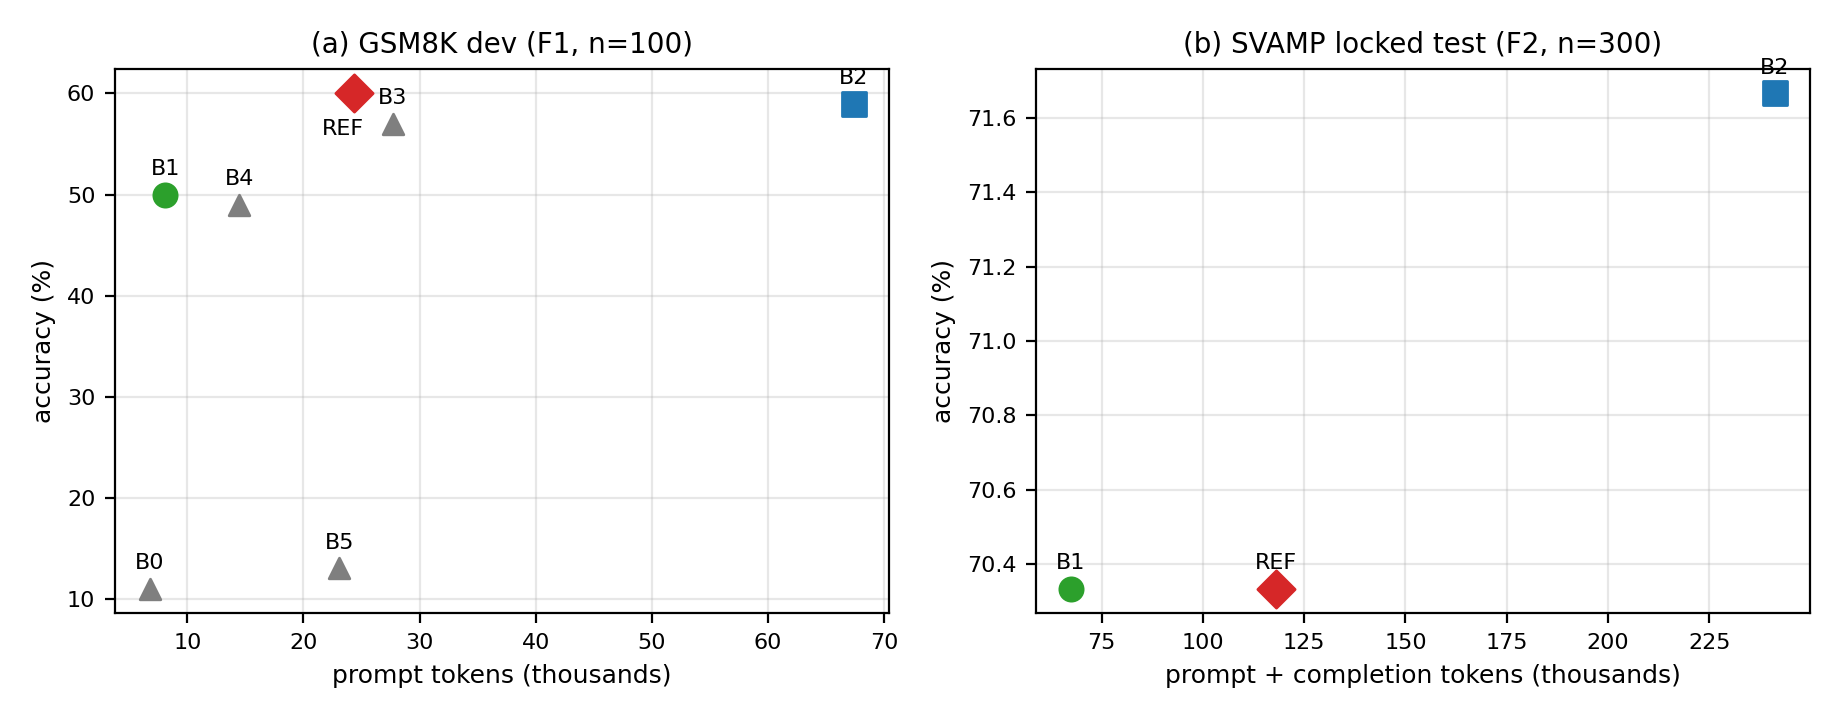
\includegraphics[width=\textwidth]{figures/fig1_capability_cost.png}
\caption{Accuracy vs.\ inference-token cost, separate panels per dataset.
(a) GSM8K dev (F1, $n{=}100$, prompt tokens): direct baselines collapse;
CoT configurations cluster at 49--60\% with ${\sim}8.3\times$ prompt-token
spread; REF shows no detectable advantage over B2 at mid-range cost. (b)
Locked SVAMP test (F2, $n{=}300$, prompt+completion tokens): B1 attains
REF's observed accuracy at the lowest cost; B2 is nominally highest in
both.}
\label{fig:scatter}
\end{figure*}

\paragraph{Non-transfer of the dev-side memory benefit.} Tier-2's REF$-$B1
point estimate ($+10.0$pp on GSM8K dev) was \emph{not replicated} on SVAMP
($0.00$pp; Figure~\ref{fig:diffs}). We state this precisely: the dev
estimate did not replicate cross-benchmark. This is not a formal
demonstration of a significant task$\times$memory interaction (contrasting
p-values is not an interaction test), not evidence of equivalence, and not
proof that memory never transfers---it is one paired, pre-locked
non-replication at $n{=}300$ resolution ($\pm{\sim}5$pp).

\begin{figure}[t]
\centering
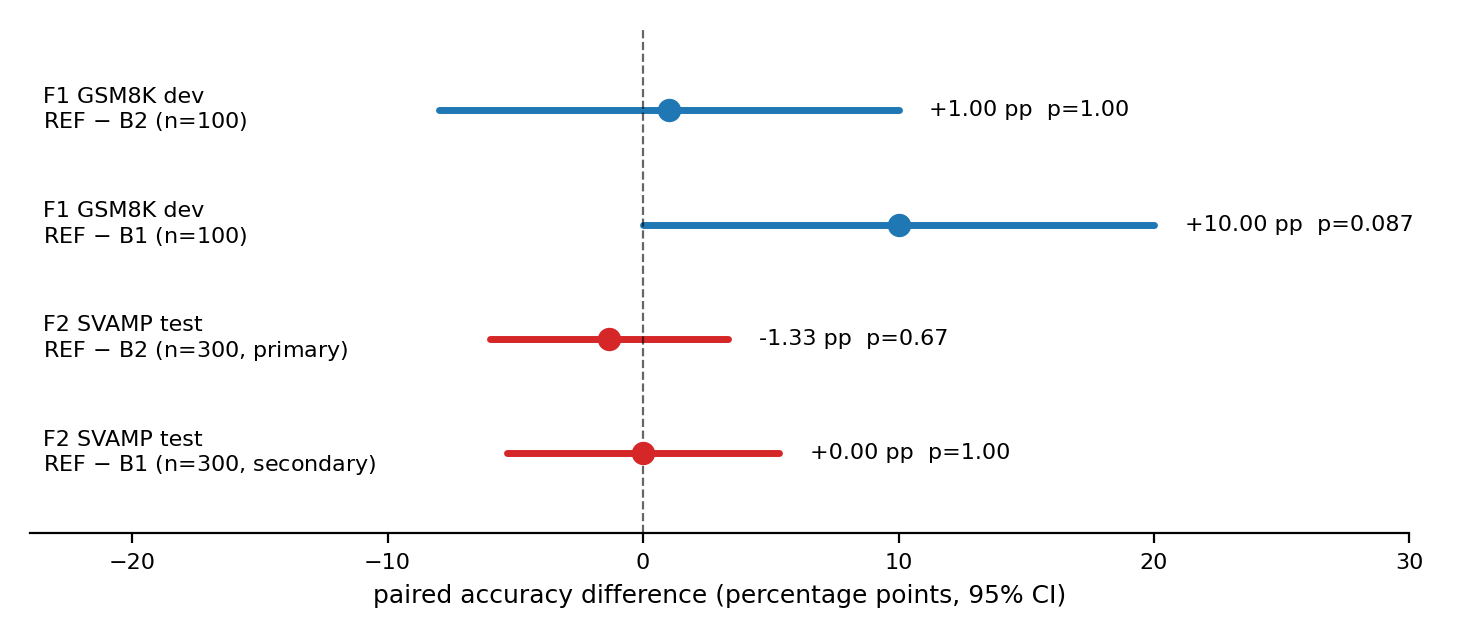
\includegraphics[width=\columnwidth]{figures/fig2_paired_diffs.png}
\caption{Paired accuracy differences with 95\% bootstrap CIs (blue: F1
GSM8K dev; red: F2 locked SVAMP test). CIs are sampling uncertainty, not
equivalence bounds: absence of a detectable difference does not establish
that the compared configurations are equal.}
\label{fig:diffs}
\end{figure}

\section{What the Evidence Supports}

\paragraph{Supported.}
(1) \emph{Cognitive configuration choices materially affect accuracy and
cost}: direct vs CoT reasoning swings GSM8K dev accuracy 11--13\%
$\rightarrow$ 49--60\%; the locked holdout gap of the searched CoT
configuration over direct fixed baselines is +29.0/+16.7pp; CoT variants
span ${\sim}8.3\times$ in prompt tokens with observed accuracies of
49--60\%, so the cost--accuracy tradeoff is configuration-dependent.
(2) \emph{Task-conditioned selection is stable and interpretable at the
family level}: CoT-dominant configurations win on GSM8K across seeds;
PubMedQA converges to no-memory direct; QASPER shifts toward retrieval
memory (pre-specified, confirmed).
(3) \emph{Search-side preferences can fail to generalize}: dev-selected
task-specific configurations lost to the GSM8K configuration on two
holdouts (Tier 1); the dev-side memory benefit did not replicate on SVAMP
(Tier 3). Held-out, fair-baseline, cross-benchmark auditing is what
separates specialization from generalizable advantage.

\paragraph{Unsupported (claimed nowhere).}
(1) \emph{Search superiority}: no detectable REF advantage over strong
presets in Tiers 2--3; evolutionary search $\approx$ equal-budget random
search on the enumerated landscape (Tier 1).
(2) \emph{Universal or scale-growing memory benefit}: effects are task-
and scale-dependent; the one pre-locked cross-benchmark test found none.
(3) \emph{Neural substrate benefit}: the trainable Mamba-2 substrate is
implemented and searchable but not selected as beneficial.

\section{Reproducibility and Ethics}

All evaluation code, locked protocols, configuration files, per-item
predictions (900/900 with full raw completions for Tier 3), statistics
scripts, the read-only forensic verifier, and figure scripts are included
in the anonymous supplementary. Tier-1 artifacts are frozen at their locked
commits; Tier 3 was pre-locked before inference and is auditable
byte-for-byte. Tiers 2--3 together used $<0.25$ GPU-hours. The work uses
public benchmarks and public models, involves no human subjects, and
reports negative results and failure modes explicitly. We release no new
model weights. The public models and benchmarks we use carry known
limitations---benchmark contamination, annotation noise, and the general
misuse potential of LLMs---and our released configurations and predictions
inherit them; we do not claim our audit protocol eliminates these risks,
and downstream users should scrutinize reused artifacts accordingly.

\section{Limitations}

Single model family (Qwen2.5, 1.5B/7B). SVAMP is a public
benchmark---pretraining contamination cannot be ruled out, and it is not
same-distribution with GSM8K, so Tier 3 is cross-benchmark rather than
i.i.d.\ confirmation. Dev slices are small ($n{=}100/50$) and were exposed
to selection (Tier 2 is exploratory; 7B and B4 contrasts are secondary and
unadjusted for multiplicity). $n{=}300$ gives $\pm{\sim}5$pp CI resolution;
absence of detectable differences is not equivalence. Tier-1 fixed
baselines were direct-only, so its headline cannot be attributed to search
alone. F1 provenance is partially undocumented (manifest coverage, runner
git SHA) and QASPER dev raw outputs were not preserved. QASPER scoring is
extraction-sensitive (marker placement), which we diagnose but do not claim
to fix. Our scaffolds are QA-style single-agent configurations; nothing
here directly addresses interactive tool-use, multi-agent, embodied, or
long-horizon agents, or backbones outside one family.

\bibliography{references}

\end{document}
